\usetikzlibrary{calc}

\begin{frame}{timing and cryptography}
    \begin{itemize}
    \item lots of asymmetric cryptography uses big-integer math
    \item example: multiplying 500+ bit numbers together
    \vspace{.5cm}
    \item how do you implement that?
    \end{itemize}
\end{frame}

\begin{frame}{big integer multiplication}
    \begin{itemize}
    \item say we have two 64-bit integers $x$, $y$
        \begin{itemize}
        \item and want to 128-bit product, but our multiply instruction only does 64-bit products
        \end{itemize}
    \item one way to multiply:
    \vspace{.5cm}
    \item divide $x$, $y$ into 32-bit parts: $x=x_1\cdot2^{32}+x_0$ and $y=y_1\cdot2^{32}+y_0$
    \item then $xy = x_1y_12^{64}+x_1y_0\cdot2^{32}+x_0y_1\cdot2^{32}+x_0y_0$
    \vspace{.5cm}
    \item<2-> can extend this idea to arbitrarily large numbers
    \item<2-> \myemph{number of smaller multiplies depends on size of numbers!}
    \end{itemize}
\end{frame}

\begin{frame}{big integers and cryptography}
    \begin{itemize}
    \item naive multiplication idea:
        \begin{itemize}
        \item number of steps depends on size of numbers
        \end{itemize}
    \item problem: sometimes the value of the number is a secret
        \begin{itemize}
        \item e.g. part of the private key
        \end{itemize}
    \item oops! revealed through timing
    \end{itemize}
\end{frame}

\begin{frame}{big integer timing attacks in practice (1)}
    \begin{itemize}
    \item early versions of OpenSSL (TLS implementation) had timing attack
        \begin{itemize}
        \item Brumley and Boneh, ``Remote Timing Attacks are Practical'' (Usenix Security '03)
        \end{itemize}
    \item attacker could figure out bits of private key from timing
    \vspace{.5cm}
    \item why? variable-time multiplication and modulus operations
        \begin{itemize}
        \item got faster/slower depending on how input was related to private key
        \end{itemize}
    \end{itemize}
\end{frame}

\begin{frame}{big integer timing attacks in practice (2)}
    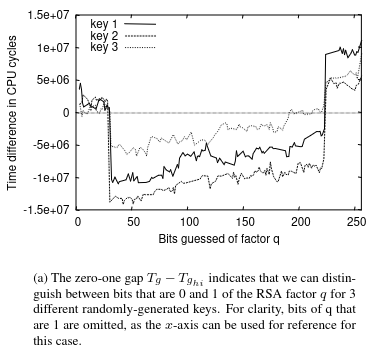
\includegraphics[height=0.9\textheight]{../spectre/remote-timing-prac-fig3a}
    \imagecredit{Figure 3a from Brumley and Boneh, ``Remote Timing Attacks are Practical''}
\end{frame}
